\documentclass[11pt,a4paper]{ctexart}
\usepackage{fontspec}
\defaultfontfeatures{Mapping=tex-text}
\usepackage{xunicode}
\usepackage{xltxtra}
%\setmainfont{???}
\usepackage{amsmath}
\usepackage{amsfonts}
\usepackage{amssymb}
\usepackage{graphicx}
\usepackage{amsthm}
\usepackage{array}
\usepackage{float}   %{H}
\usepackage{booktabs}  %\toprule[1.5pt]
\usepackage[titletoc]{appendix}
\usepackage{tcolorbox} %彩色框框
%===================%插入代码需要的控制
\usepackage{listings}
\usepackage{xcolor}
\setmonofont{Consolas}%字体
\lstset{
	numbers=left, 
	numberstyle= \tiny, 
	keywordstyle= \color{ blue!70},
	commentstyle= \color{red!50!green!50!blue!50}, 
	frame=shadowbox, % 阴影效果
	rulesepcolor= \color{ red!20!green!20!blue!20} ,
	escapeinside=``,% 英文分号中可写入中文
	breaklines=true,
	basicstyle=\ttfamily 
} 
%===================%
\usepackage[left=2cm,right=2cm,top=2cm,bottom=2cm]{geometry}

\newtheorem{theorem}{定理}
\newtheorem{definition}{定义}
\newtheorem*{solution}{解}

\title{定性数据统计分析作业 (7)}
\author{钟瑜 \quad 222018314210044}
\date{\today}
\begin{document}
\maketitle
\pagestyle{plain}%设置页码
%================================================================%
\begin{figure}[H]
	\centering
	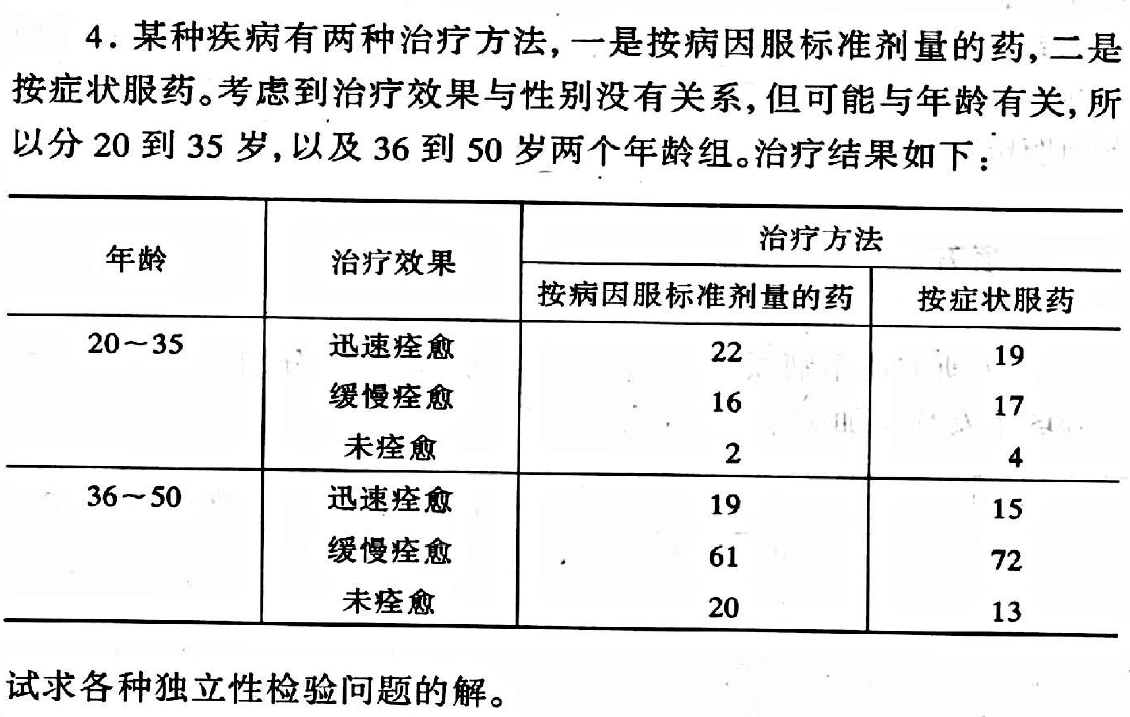
\includegraphics[width=0.7\textwidth]{screenshot002}
	\label{fig:screenshot002}
\end{figure}

\begin{solution}
计算独立性检验的p值:
\end{solution}
\begin{lstlisting}[language=r]
> #高维列联表独立性检验
> mut_independence=function(x){
+   r=dim(x)[1];r    #行
+   c=dim(x)[2];c    #列
+   t=dim(x)[3];t    #层
+   n=sum(x)
+   temp11=0
+   temp21=0
+   temp22=0
+   temp23=0
+   temp31=0
+   temp32=0
+   temp33=0
+   for (i in 1:r) {
+     for (j in 1:c){
+       for (k in 1:t){
+         ni__=sum(x[i,,])
+         n_j_=sum(x[,j,])
+         n__k=sum(x[,,k])
+         n_jk=sum(x[,j,k])
+         ni_k=sum(x[i,,k])
+         nij_=sum(x[i,j,])
+         temp11=temp11+x[i,j,k]*log(ni__*n_j_*n__k/(x[i,j,k]*n^2))
+         
+         temp21=temp21+x[i,j,k]*log(ni__*n_jk/(x[i,j,k]*n))
+         temp22=temp22+x[i,j,k]*log(n_j_*ni_k/(x[i,j,k]*n))
+         temp23=temp23+x[i,j,k]*log(n__k*nij_/(x[i,j,k]*n))
+         
+         temp31=temp31+x[i,j,k]*log(ni_k*nij_/(x[i,j,k]*ni__))
+         temp32=temp32+x[i,j,k]*log(nij_*n_jk/(x[i,j,k]*n_j_))
+         temp33=temp33+x[i,j,k]*log(ni_k*n_jk/(x[i,j,k]*n__k))
+         	
+       }
+     }
+   }
+   A_B_C=-2*temp11;A_B_C
+   A_BC=-2*temp21;A_BC
+   B_AC=-2*temp22;B_AC
+   C_AB=-2*temp23;C_AB
+   AB_AC=-2*temp31;AB_AC
+   BA_BC=-2*temp32;BA_BC
+   CA_CB=-2*temp33;CA_CB
+   
+   cat('\n(A,B,C) p值:',1-pchisq(A_B_C, r*c*t-r-c-t+2))
+   cat('\n(A,BC)  p值:',1-pchisq(A_BC, (r-1)*(c*t-1)))
+   cat('\n(B,AC)  p值:',1-pchisq(B_AC, (c-1)*(r*t-1)))
+   cat('\n(C,AB)  p值:',1-pchisq(C_AB, (t-1)*(r*c-1)))
+   cat('\n(AB,AC) p值:',1-pchisq(AB_AC, r*(c-1)*(t-1)))
+   cat('\n(BA,AC) p值:',1-pchisq(BA_BC, c*(r-1)*(t-1)))
+   cat('\n(CA,CB) p值:',1-pchisq(CA_CB, t*(r-1)*(c-1)))
+ }
> dim(x)=c(3,2,2);x
, , 1

[,1] [,2]
[1,]   22   19
[2,]   16   17
[3,]    2    4

, , 2

[,1] [,2]
[1,]   19   15
[2,]   61   72
[3,]   20   13

> mut_independence(x)

(A,B,C) p值: 5.943482e-06
(A,BC)  p值: 2.246753e-06
(B,AC)  p值: 0.5773336
(C,AB)  p值: 2.083189e-06
(AB,AC) p值: 0.6496818
(BA,AC) p值: 6.493699e-07
(CA,CB) p值: 0.4325714
\end{lstlisting}

(A,B,C) p值: 5.943482e-06\\
(A,BC)  p值: 2.246753e-06\\
(B,AC)  p值: 0.5773336\\
(C,AB)  p值: 2.083189e-06\\
(AB,AC) p值: 0.6496818\\
(BA,AC) p值: 6.493699e-07\\
(CA,CB) p值: 0.4325714\\

可以看出,A,B 和C 之间仅有相关关系。它们相互之间不独立,其中任意一个和另外两个也不独立,其中任意一个给定后另外两个条件独立。(B,AC)  p值: 0.57733>0.1  不独立,B与AC相关.

\begin{figure}[H]
	\centering
	
\includegraphics[width=0.7\textwidth]{screenshot003}
	\label{fig:screenshot003}
\end{figure}
\begin{figure}[H]
	\centering
	
\includegraphics[width=0.7\textwidth]{screenshot004}
	\label{fig:screenshot004}
\end{figure}


\begin{solution}
\end{solution}
\begin{lstlisting}[language=r]
congruence_test=function(x,alternative="twoside")
#适用于列联表的相合性检验问题
#x为列联表矩阵;alternative对应于备择假设'twoside'相合,'greater'正相合,or'less'负相合
{
	n=sum(x)
	G=0;H=0
	r=nrow(x)
	c=ncol(x)
	r1=r-1;c1=c-1
	for (i in 1:r1){
		for (j in 1:c1){
			G=G+x[i,j]*sum(x[(i+1):r,(j+1):c])
		}
	}
	for (i in 1:r1){
		for (j in 2:c){
			H=H+x[i,j]*sum(x[(i+1):r,1:(j-1)])
		}
	}
	z=G-H
	TA=sum(rowSums(x)*(rowSums(x)-1)/2)
	TB=sum(colSums(x)*(colSums(x)-1)/2)
	#TAB=G+H+TA+TB-n*(n-1)/2
	Cn2=n*(n-1)/2
	#计算各系数的值
	Kendall_TAO=z/sqrt((Cn2-TA)*(Cn2-TB))
	Gamma=(G-H)/(G+H)
	d_BA=(G-H)/(Cn2-TA)
	d_AB=(G-H)/(Cn2-TB)
	
	#近似公式,表示sigma的平方
	sigma_2=(n^3-sum(rowSums(x)^3))*(n^3-sum(colSums(x)^3))/(9*n^3) 
	
	#构建U统计量
	U=z/sqrt(sigma_2)
	if(alternative=="twoside")
	{p_value=1-pchisq(U^2, 1)}
	else 
	{
		if(alternative=="greater")
		{p_value=pnorm(-U)}
		else if(alternative=="less")
		{p_value=pnorm(U)}
		else{cat("please input:\n alternative= 'twoside','greater',or'less'")}
	}
	cat('【各种相关系数】\n')
	cat('Kendall_TAO=',Kendall_TAO,'\n')
	cat('Gamma=',Gamma,'\n')
	cat('d_BA=',d_BA,'\n')
	cat('d_AB=',d_AB,'\n\n')
	cat('【相合性检验】\n')
	cat('U检验统计量的值',U,'\n')
	cat('p_value=',p_value)
}

> x=c(37,11,26,23,30,31,43,11)
> dim(x)=c(2,2,2);x
, , 1

[,1] [,2]
[1,]   37   26
[2,]   11   23

, , 2

[,1] [,2]
[1,]   30   43
[2,]   31   11

> mut_independence(x)        

(A,B,C) p值: 0.001036864
(A,BC)  p值: 0.0004155325
(B,AC)  p值: 0.0003747595
(C,AB)  p值: 0.0005111978
(AB,AC) p值: 0.0001482043
(BA,AC) p值: 0.0001652176
(CA,CB) p值: 0.0001191498

> #各个独立性检验的p值都很小,故这三个属性相互之间仅有相关关系
> #下对年龄进行分层,讨论相合性
> A1=x[,,1]
> A2=x[,,2]

> congruence_test(A1,alternative="greater")
【各种相关系数】
Kendall_TAO= 0.2517214 
Gamma= 0.4969217 
d_BA= 0.2637722 
d_AB= 0.2402211 

【相合性检验】
U检验统计量的值 2.479168 
p_value= 0.006584467

> #拒绝原假设,认为是正相合,即年轻人中,男性偏好饮料A,女性偏好饮料B
> congruence_test(A2,alternative="less")
【各种相关系数】
Kendall_TAO= -0.3156117 
Gamma= -0.6031269 
d_BA= -0.3271363 
d_AB= -0.304493 

【相合性检验】
U检验统计量的值 -3.384558 
p_value= 0.0003564646
> #拒绝原假设,认为是负相合,及老年人中,男性偏好饮料B,女性偏好饮料A

\end{lstlisting}


\end{document}